\title{Chapter 4, Section 4. Exercises 1, 2, and 4.}
\author{
	MTH 594, Prof. Mikael Vejdemo-Johansson \\
	Differential Geometry Independent Study \\
	\\
	Matthew Connelly \\
}
\date{\today}



\documentclass[12pt]{article}

\usepackage[top=.5in, bottom=.75in, left=1in, right=1in]{geometry}
\usepackage{amssymb}
\usepackage{amsmath}
\usepackage{graphicx}
\usepackage{subcaption}

\newcommand{\ulind}[1]
{
\noindent
\underline{#1}\\\\
\indent
}

\newcommand{\R}
{
\mathbb{R}
}

\begin{document}
\maketitle

\section*{Exercise 11.1.1}
\indent

Show that, if $l$ is a half-line geodesic in $\mathbb{H}$ and $a$ is a point not on $l$, there are infinitely  many hyperbolic lines passing through $a$ that do not intersect $l$.

\vspace{1cm}
\hrule
\vspace{1cm}
\noindent

\ulind{Preliminary Statements}

Euclid's parallel postulate states that, in euclidean geometry, if there is a point $p$ not on a line $l$, there is exactly one line parallel to $l$ going through $p$.

\begin{figure}[h!]
  \centering
      \begin{subfigure}[b]{0.37\linewidth}
    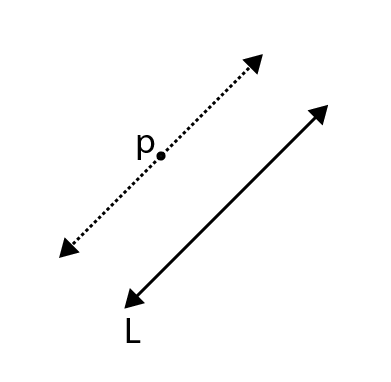
\includegraphics[width=\linewidth]{./assets/11-1-1/parallel-postulate.png}
  \end{subfigure}
  \end{figure}
  \indent

\clearpage

This is not true in hyperbolic geometry; rather, there are infinitely many lines parallel to $l$ passing through $p$.

\begin{figure}[h!]
  \centering
      \begin{subfigure}[b]{0.5\linewidth}
    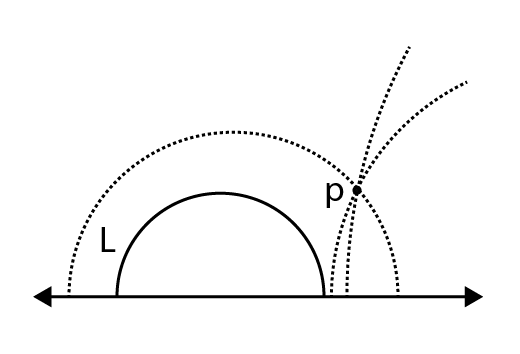
\includegraphics[width=\linewidth]{./assets/11-1-1/parallel-postulate-hyperbolic.png}
  \end{subfigure}
  \end{figure}
  \indent

\ulind{Solution}

Let $l$ meet the real axis at point $b$, and let the real component of $a > b$.\\\\

\begin{figure}[h!]
  \centering
      \begin{subfigure}[b]{0.75\linewidth}
    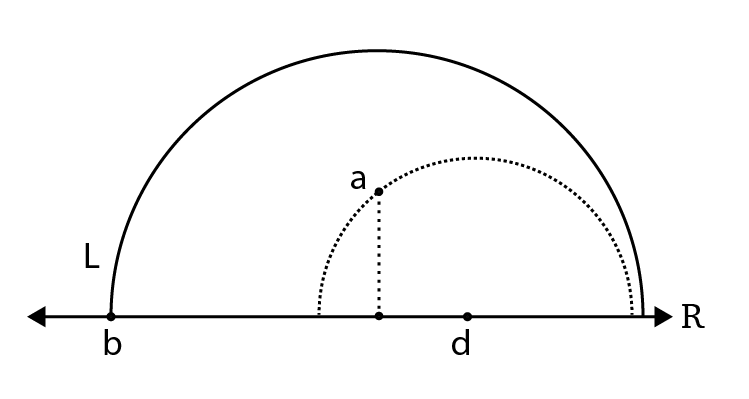
\includegraphics[width=\linewidth]{./assets/11-1-1/non-intersecting.png}
  \end{subfigure}
  \end{figure}
  \indent
  
The semicircle with a center $d$ on the real axis and radius $|a - d|$ passes through $a$ and does not meet  $l$ if $|a - d| \leq |d-b|$.

\end{document}
